\documentclass{beamer}

\usepackage{beamerthemesplit}
\usepackage{verbatim}

\usetheme{Pittsburgh}
%\usecolortheme{seagull}
%\usecolortheme{seahorse}
\usecolortheme{beaver}

\usefonttheme{serif}

\newcommand{\snT}{$(S/N)_{\textrm{size}}$}
%\newcommand{\snT}{$\left( \frac{S}{N}\right)_{\textrm{size}}$}
\newcommand{\snflux}{$(S/N)_{\textrm{flux}}$}
%\newcommand{\snflux}{$\left( \frac{S}{N}\right)_{\textrm{flux}}$}

\newcommand{\lensfit}{\texttt{LENSFIT}}
\newcommand{\numba}{\texttt{Numba}}
\newcommand{\python}{\texttt{Python}}
\newcommand{\ngmix}{\texttt{ngmix}}
\newcommand{\shear}{{\bf g}}

\title{Bayesian Shear Estimation}
\author{Erin Sheldon}
\institute{Brookhaven National Laboratory}

% http://texblog.net/latex-archive/plaintex/beamer-footline-frame-number/
% to add the page (frame ) number and not screw up the bottom line
% works for split themes?
\expandafter\def\expandafter\insertshorttitle\expandafter{%
      \insertshorttitle\hfill%
        \insertframenumber\,/\,\inserttotalframenumber}


\begin{document}

\frame{\titlepage}

\section{Introduction}

\frame
{
    \frametitle{Shear}

    \begin{itemize}

        \item Weak shear is smaller than the intrinsic variance in shapes.
            
        \item We average the shear from many sources to extract a signal.

        \item Look for correlations in the shear field, or between shear and
            known objects positions.


    \end{itemize}
}
\frame
{
    \frametitle{Shear}
    \fontsize{9}{0.8\baselineskip}

    \begin{columns}
        \begin{column}{0.5\textwidth}
            \begin{itemize}

                \item Correlations in the shear/matter field hold information
                    about the {\bf Dark Matter} distribution.  The Cold Dark
                    Matter theory predicts these correlations and the
                    corresponding shear correlations.

                \item The theory does {\bf not } predict the structure of
                    individual dark matter halos.  A weak shear measurement in
                    the direction of a single object is just a poorly measured
                    and difficult to interpret shear correlation function.

            \end{itemize}
        \end{column}

        \begin{column}{0.5\textwidth}
            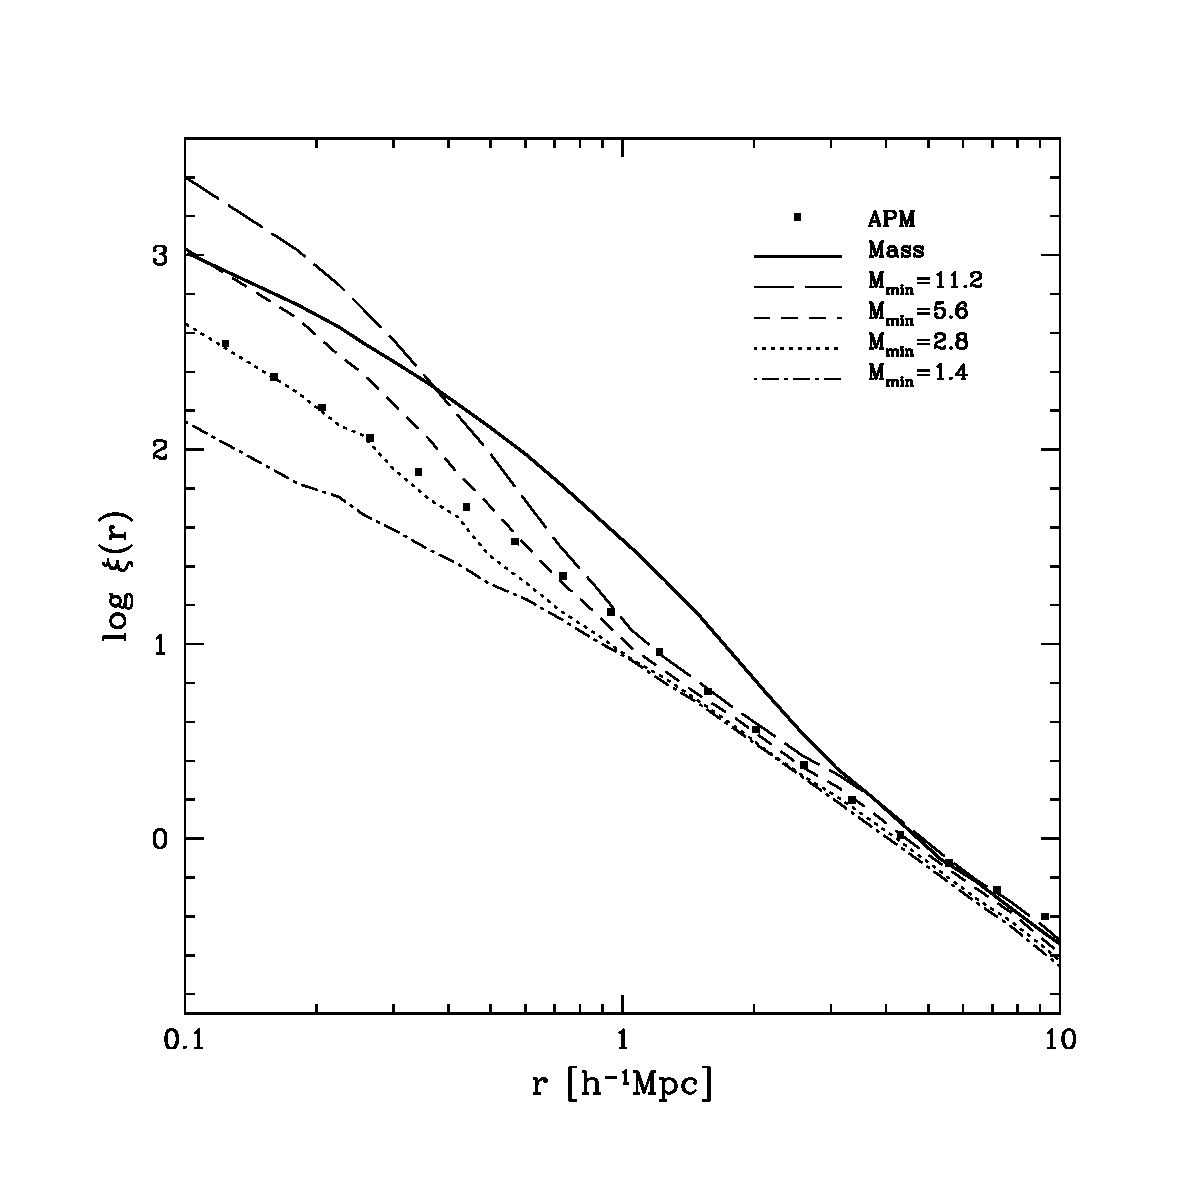
\includegraphics[width=\textwidth]{berlind-weinberg-f3.pdf}
            \newline
            \begin{center}
                {\tiny Berlind \& Weinberg 2002}
            \end{center}
        \end{column}
    \end{columns}
}

%                \item To meet goals of current surveys we want to measure shear
%                    to about 0.4\% accuracy (e.g.  Dark Energy Survey).  LSST a
%                    factor of a few better.



\frame
{
    \frametitle{Shear Measurements}
    
    \begin{itemize}

        \item Forward-modeling: Fit a model that is convolved by an estimate of
            the PSF. Limited by how well one can model the galaxy and PSF (e.g.
            Miller et al., Bernstein \& Armstrong, many others).

        \item Moments: Measure moments and correct them for the PSF.  Use a
            weight function to suppress the noise. Derive how that measurement
            responds to smearing by the PSF and shearing (e.g.  Kaiser,
            Squires, \& Broadhurst, Bernstein \& Jarvis, Melchior, Bernstein \&
            Armstrong).  Working in Fourier space can help with the
            deconvolution (Bernstein).

        \item These methods can be made to work well, as long as the $S/N$ is
            still pretty high, say 50 or higher.

    \end{itemize}
}

\frame
{
    \frametitle{Noise Bias}

    \begin{itemize}

        \item Non-linear fitting in the presence of noise is biased, both the
            maximum likelihood and expectation value over the posterior: using
            the mean shape won't work (Hirata, Refregier, etc).   Results in a
            {\bf calibration} error.

        \item This is generally known in statistics, but not yet solved for our
            particular problem. Badly aggravated by the PSF ``deconvolution''.

        \item The noise also causes problems for moment based methods.

    \end{itemize}
}

\frame
{
    \frametitle{Maximum Likelihood}

    \begin{center}
    \includegraphics[width=0.7\textwidth]{{gmix-fit-gg05r01-yr-0.005-0.005-diff}.pdf}
\end{center}

}

\section{Bayesian Methods}

\frame
{
    \begin{center}
        {\huge Bayesian Shear Measurement }
    \end{center}
}

\frame
{
    \frametitle{Miller et al. 2007}

    \begin{itemize}

        \item Miller et al. 2007 (\lensfit): Use priors on the parameters and
            explore a constrained posterior surface (Prior $\times$
            Likelihood).

        \item Attempt to derive how the shear estimate (the shape) affected by
            the noise and prior using integrals over the posterior surface and
            first order approximation in shear.  Called the {\bf response}.

        \item The posterior surface of the shape for a single galaxy is
            complex.  The space is bounded, the surface is necessarily
            asymmetric and depends on galaxy properties and noise.

        \item No rigorous expression is given for the mean shear of a
            population given these ellipticity responses.  Choose to simply
            average them.

        \item Miller et al. 2013 find large biases in simulations, of
            order 10\% at \snflux$ \sim 10$.
        
    \end{itemize}
}

\begin{comment}
\frame
{
    \frametitle{Miller et al. 2007}

    Assume a small shear $g$ just shifts the likelihood a small amount.
    Taylor expand
    \begin{eqnarray}
        L(g) & \rightarrow & L(g - \gamma_{\mu}) \\
             & \approx     & L(g) - \gamma_{\mu} \frac{ \partial L }{ \partial g_{\mu} } + . . .
    \end{eqnarray}
}
\end{comment}

\frame
{
    \frametitle{\lensfit\ Tests}

    \begin{columns}
        
        \begin{column}{0.5\textwidth}
            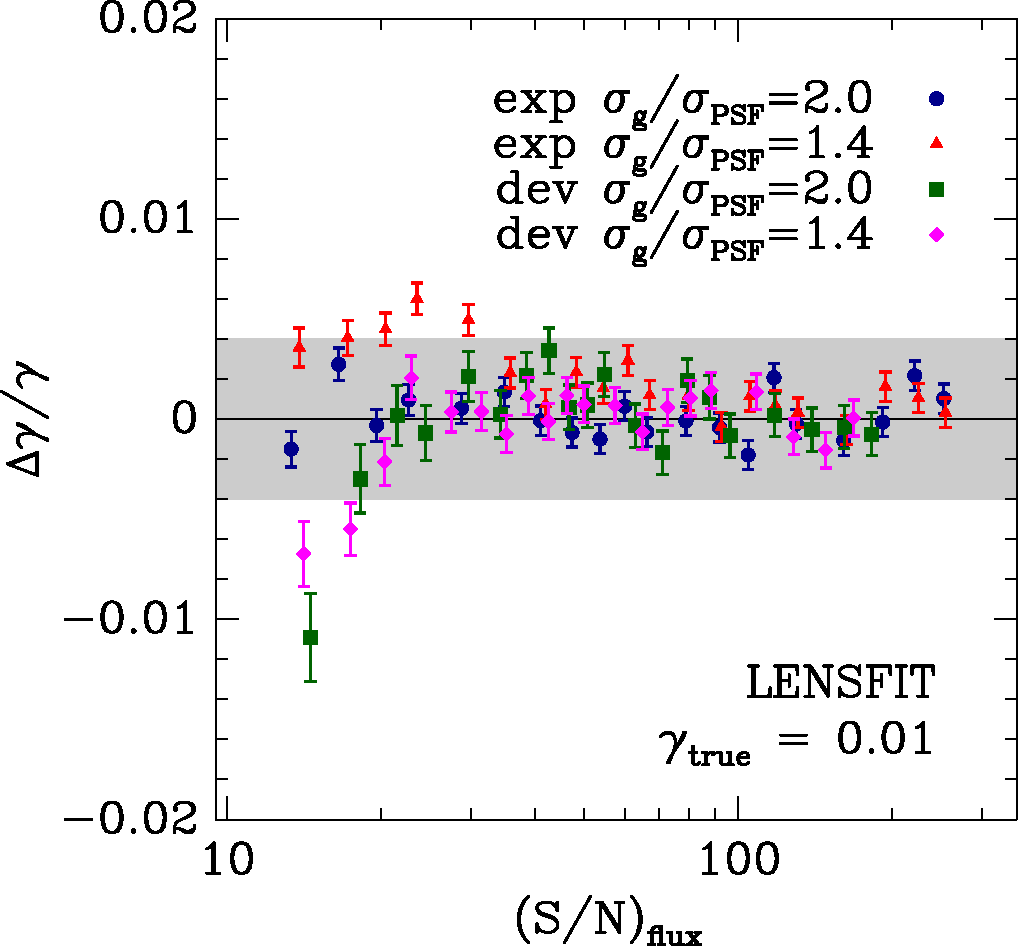
\includegraphics[width=\textwidth]{cbafit-geg07-geg08-deg03-deg05-lensfit-flux-s2n.pdf}
        \end{column}

        \begin{column}{0.5\textwidth}
            \includegraphics[width=\textwidth]{cbafit-geg07-geg08-deg03-deg05-lensfit-T-s2n.pdf}
        \end{column}
    \end{columns}

    \fontsize{9}{0.8\baselineskip}
    \begin{itemize}

        \item I did my own tests of \lensfit\ with strong structural priors
            (30\% lognormal on flux, 15\% on size (that was a bug...) ).

        \item Very fast code using gaussian mixtures to approximate galaxies.  Fast
            analytic convolutions.

        \item Bias vs \snT\ has more universal form than vs \snflux.
    \end{itemize}

}

\begin{comment}
\frame
{
    \frametitle{Shear of the Light Distribution}

    \begin{itemize}

        \item Stack the light around peaks in images.

        \item Assume the shear is constant over the patch of interest.

        \item This two-dimensioinal correlation function of the light is
            sheared just as galaxy images are.  Don't need to de-blend.  Not
            fully explored (ES).

    \end{itemize}
}
\end{comment}

\frame
{
    \frametitle{Bernstein \& Armstrong 2013}

    \begin{itemize}

        \item Shape is not shear.
        \item While the posterior surface for the {\it shape} of single galaxy
            is complex, the posterior surface for the {\it mean shear} of an
            ensemble must approach a Gaussian according to the central limit
            theorem.  This is both useful and actually true!

         \item Assuming Gaussianity, weak shear, and knowledge of underlying
             distribution of shapes for the ensemble (the prior), one can
             derive an unbiased estimator for the mean shear of the ensemble.

         \item You lose nothing: in the limit of weak shear, you need
             to use an ensemble statistic anyway.  The ``shape noise'',
             intrinsic variance in shapes of galaxies, dominates over
             the signal.

        \item This is a good idea, but needed an implementation, so I worked it
            into my existing code.
         
    \end{itemize}

}

\frame
{
    \frametitle{Bernstein \& Armstrong}

    Assume a small shear \shear.  The posterior probability for
    the shear estimated from many galaxies
    \begin{eqnarray}
    P(\shear | {\bf D}) & = & \frac{ P(\shear) P({\bf D}|\shear ) }{ P({\bf D}) }  \\
                        & = & P(\shear) \prod_i \frac{ P({\bf D}_i | \shear) }{ P({\bf D}_i) } \\
        P({\bf D}_i | \shear) & \approx & P_i + \shear  \cdot {\bf Q}_i + \frac{1}{2} \shear \cdot {\bf R}_i \cdot \shear
    \end{eqnarray}
}



\frame
{
    \frametitle{Bernstein \& Armstrong Tests}

    \begin{columns}
        
        \begin{column}{0.5\textwidth}
            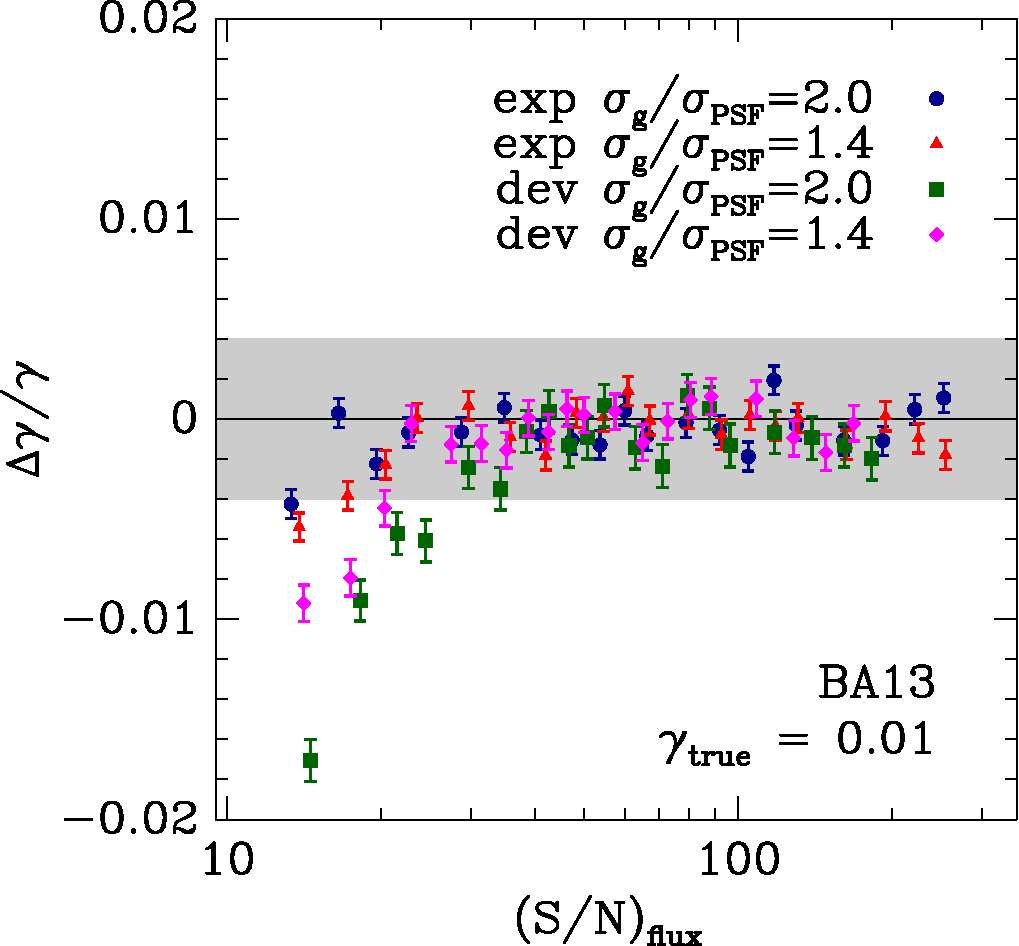
\includegraphics[width=\textwidth]{cbafit-geg07-geg08-deg03-deg05-ba13-flux-s2n.pdf}
        \end{column}

        \begin{column}{0.5\textwidth}
            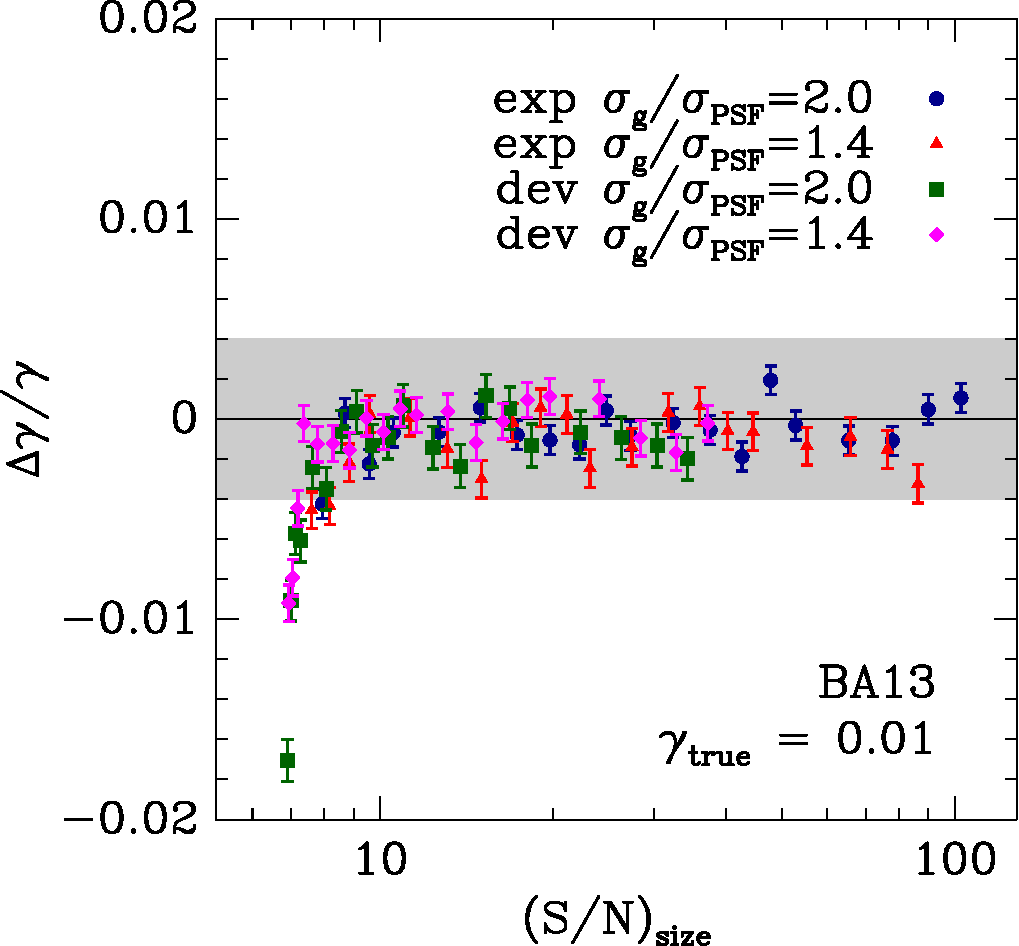
\includegraphics[width=\textwidth]{cbafit-geg07-geg08-deg03-deg05-ba13-T-s2n.pdf}
        \end{column}
    \end{columns}

    \begin{itemize}
        \item Assuming we can find the right model.
        \item Sufficient accuracy for DES at \snT$ > 10$.
    \end{itemize}
}


\frame
{
    
    \frametitle{Bernstein \& Armstrong Tests}

    \begin{itemize}
        \item Can push to lower \snT\ than \lensfit.

        \item Bias varies with \snT\ in a simpler way than \lensfit.
        \item Bias vs \snT\ even more universal. Sufficient accuracy for DES at \snT$ > 10$.

       

    \end{itemize}
}

\frame
{
    \frametitle{Limitations}
    \begin{itemize}

        \item I'm assuming I can find the right model.  Not true in real data.
            Should be OK for DES (Kacprzak et al. 2013) but not LSST.

        \item TODO: 
            
            \begin{itemize}

                \item Why is there bias at all?  Is it the likelhood sampling
                    method?

                \item For real data need a shape prior that is twice
                    differentiable.

                \item Bernstein \& Armstrong propose a model-independent
                    technique using moments in Fourier space, but not yet
                    implemented.  Gary and Bob plan to do it.  Student at Stony
                    Brooke as well (Madhavacheril).

            \end{itemize}

    \end{itemize}
}

\frame
{
    \frametitle{The Code}

    \begin{itemize}

        \item The code is fairly mature.  New version \ngmix\ re-written using
            {\texttt \python + \numba}.

        \item On github  \texttt{https://github.com/esheldon/ngmix}. 
            
        \item The old version \texttt{gmix\_image} doesn't require \numba.
            Also available, but is no longer maintained.

        \item The code is running on DES data, measuring multi-epoch and
            multi-band shears and fluxes.  
            
        \item Need to determine shape prior that is twice differentiable.

    \end{itemize}
}
\frame
{
    \frametitle{Summary}

    \begin{itemize}

        \item Shear estimation is difficult in the presence of noise.

        \item Modern techniques can work well enough for current surveys.

        \item For future experiments such as LSST may need a model-independent
            approach.

    \end{itemize}
}

\end{document}
